%
% File acl2021.tex
%
%% Based on the style files for EMNLP 2020, which were
%% Based on the style files for ACL 2020, which were
%% Based on the style files for ACL 2018, NAACL 2018/19, which were
%% Based on the style files for ACL-2015, with some improvements
%%  taken from the NAACL-2016 style
%% Based on the style files for ACL-2014, which were, in turn,
%% based on ACL-2013, ACL-2012, ACL-2011, ACL-2010, ACL-IJCNLP-2009,
%% EACL-2009, IJCNLP-2008...
%% Based on the style files for EACL 2006 by 
%%e.agirre@ehu.es or Sergi.Balari@uab.es
%% and that of ACL 08 by Joakim Nivre and Noah Smith

\documentclass[11pt,a4paper]{article}
\usepackage[hyperref]{acl2021}
\usepackage{times}
\usepackage{latexsym}
\renewcommand{\UrlFont}{\ttfamily\small}
\usepackage{graphicx}

% This is not strictly necessary, and may be commented out,
% but it will improve the layout of the manuscript,
% and will typically save some space.
\usepackage{microtype}

%\aclfinalcopy % Uncomment this line for the final submission
%\def\aclpaperid{***} %  Enter the acl Paper ID here

%\setlength\titlebox{5cm}
% You can expand the titlebox if you need extra space
% to show all the authors. Please do not make the titlebox
% smaller than 5cm (the original size); we will check this
% in the camera-ready version and ask you to change it back.

%\newcommand\BibTeX{B\textsc{ib}\TeX}


\usepackage{biblatex} %Imports biblatex package
\addbibresource{Shakespeare Text Generation.bib} %Import the bibliography file
\addbibresource{sample.bib}

\begin{document}

\title{Shakespearean Text Generation Report}

\author{  R. Chen \\\and F. Pearson \\\and J. Ressler \\\and E. Weisman }
%  \texttt{email@domain} \\\And
 % Second Author \\
  %Affiliation / Address line 1 \\
  %Affiliation / Address line 2 \\
  %Affiliation / Address line 3 \\
  %\texttt{email@domain} \\}

%\author{
%\begin{tabular}[t]{c@{\extracolsep{8em}}c} 
%R. Chen & F. Pearson & J. Ressler & E. Weisman 
%\end{tabular}
%}


\maketitle



\date{11/23/2022}

\begin{abstract}
Natural Language Processing has evolved in a multitude of way, and sees use in many facets of modern life. It also exists as a stark pillar of modernity within computer science. In contrast to this, the writings of William Shakespeare are iconic relics from a prior millennia. We asked the question: "Can current modern methods reproduce plausible results when attempting to extend Shakespeare's corpora?" In pursuit of this question, a model was built and used to provide a host of 'Shakespearean' text, which was evaluating by human elements, alongside other similar models, to evaluate the results in a non-biased manner. The process begins with the creation of a corpus of Shakespeare's plays, which are then used to generate new lines of dialogue in an attempt to reproduce the original wording as closely as possible. This technique has been applied successfully to both prose and poetry.

\end{abstract}

\section{Credits}
This document has been adapted by Roberto Navigli from the instructions for earlier ACL, NAACL and EMNLP proceedings, including those for EMNLP 2020 by Yulan He, ACL 2020 by Steven Bethard, Ryan Cotterrell and Rui Yan, ACL 2019 by Douwe Kiela and Ivan Vulic, NAACL 2019 by Stephanie Lukin and Alla Roskovskaya, ACL 2018 by Shay Cohen, Kevin Gimpel, and Wei Lu, NAACL 2018 by Margaret Michell and Stephanie Lukin, 2017/2018 (NA)ACL bibtex suggestions from Jason Eisner, ACL 2017 by Dan Gildea and
Min-Yen Kan, NAACL 2017 by Margaret Mitchell, ACL 2012 by Maggie Li and Michael White, ACL 2010 by Jing-Shing Chang and Philipp Koehn, ACL 2008 by Johanna D. Moore, Simone Teufel, James Allan, and Sadaoki Furui, ACL 2005 by Hwee Tou Ng and Kemal Oflazer, ACL 2002 by Eugene Charniak and Dekang Lin, and earlier ACL and EACL formats written by several people, including John Chen, Henry S. Thompson and Donald Walker. Additional elements were taken from the formatting instructions of the International
Joint Conference on Artificial Intelligence and the Conference. 

\section{Introduction}
\label{sec:intro}
%project goals should be well described here
We have spent our time with the development of a natural language generator, with the explicit purpose of generating legible text in a Shakespearean format. To accomplish this, we built a model, with guidance from multiple online sources to generate text based off a brief prompt. The AI model then outputs what it believe to be appropriate characters and words, to form Shakespearean text. When building the generation model, we attempted both a LTSM and GRU approach. In the end we opted to go with the GRU approach, as it had an expedient run-time and produced seemingly superior results. In order to test the validity of our model, we implemented a brief questionnaire using google forms, which was supplied to peers, friends, and family. In this questionnaire, we posed various texts, either from Shakespeare himself, or generated by our or another model. The respondents were not given information on the source of the texts. The respondents were then asked to rate the given text on a scale of one to ten, with one being the least like Shakespeare and ten being the most like Shakespeare. \\
In the pages to follow, we evaluate and explicate our data, and will determine the success of both our model in comparison to the others, as well as to the source material. Following this, we evaluate the general success text generation on producing Shakespearean English. As an added exercise, we examined text generated based off other creative commons literature using our model, although this was not evaluated on a large scale.



\section{Process Breakdown}
\label{sec:process}
%describe what NLP tasks do we address
Deleted code is debugged code. (Jeff Sickel) Every operating system out there is about equal… We all suck. (Microsoft senior vice president Brian Valentine describing the state of the art in OS security, 2003) Programming is like sex: one mistake and you’re providing support for a lifetime. (Michael Sinz) Fine, Java MIGHT be a good example of what a programming language should be like. But Java applications are good examples of what applications SHOULDN’T be like. (pixadel) Hardware: The parts of a computer system that can be kicked. (Jeff Pesis)

\section{Data and Usage}

\subsection{History of Shakespearean Text Generation}
\label{sec:history}





\subsection{The Other Models}
\label{sec:others}
Deleted code is debugged code. (Jeff Sickel) Every operating system out there is about equal… We all suck. (Microsoft senior vice president Brian Valentine describing the state of the art in OS security, 2003) Programming is like sex: one mistake and you’re providing support for a lifetime. (Michael Sinz) Fine, Java MIGHT be a good example of what a programming language should be like. But Java applications are good examples of what applications SHOULDN’T be like. (pixadel) Hardware: The parts of a computer system that can be kicked. (Jeff Pesis)

\subsection{Our Model}
\label{sec:ours}

Deleted code is debugged code. (Jeff Sickel) Every operating system out there is about equal… We all suck. (Microsoft senior vice president Brian Valentine describing the state of the art in OS security, 2003) Programming is like sex: one mistake and you’re providing support for a lifetime. (Michael Sinz) Fine, Java MIGHT be a good example of what a programming language should be like. But Java applications are good examples of what applications SHOULDN’T be like. (pixadel) Hardware: The parts of a computer system that can be kicked. (Jeff Pesis)

\subsection{The Results}
\label{sec:results}

\begin{figure}
\centering
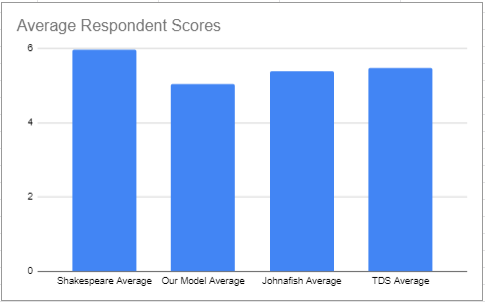
\includegraphics[width=.5\textwidth]{report/avgScores.png}
\caption{\label{fig:AverageScores}A bar chart showing the averages of scores by sources.}
\end{figure}

As can be observed under \ref{fig:AverageScores} our model performs slightly under the other two models. Given that the John Fish model operates on GRU and the Towards Data Science Model is using an LSTM, we can surmise that our under-performance is not necessarily due to model selection. That does not mean model choice was not a factor, as the lower average of the John Fish could hint to a slightly inferior performance from a GRU system. Our testing reflected this, however we chose a GRU system, as the impact to performance an LSTM had was not worth the slight increase to results we observed. 
That said, all models performed similarly well, and not drastically behind the performance of Shakespeare's writings (functionally our control).

\section{Section 7}
\label{sec:supplementary}

Deleted code is debugged code. (Jeff Sickel) Every operating system out there is about equal… We all suck. (Microsoft senior vice president Brian Valentine describing the state of the art in OS security, 2003) Programming is like sex: one mistake and you’re providing support for a lifetime. (Michael Sinz) Fine, Java MIGHT be a good example of what a programming language should be like. But Java applications are good examples of what applications SHOULDN’T be like. (pixadel) Hardware: The parts of a computer system that can be kicked. (Jeff Pesis)

\section{Section 8}
\label{ssec:accessibility}

Deleted code is debugged code. (Jeff Sickel) Every operating system out there is about equal… We all suck. (Microsoft senior vice president Brian Valentine describing the state of the art in OS security, 2003) Programming is like sex: one mistake and you’re providing support for a lifetime. (Michael Sinz) Fine, Java MIGHT be a good example of what a programming language should be like. But Java applications are good examples of what applications SHOULDN’T be like. (pixadel) Hardware: The parts of a computer system that can be kicked. (Jeff Pesis)

\section{Section 9}

Deleted code is debugged code. (Jeff Sickel) Every operating system out there is about equal… We all suck. (Microsoft senior vice president Brian Valentine describing the state of the art in OS security, 2003) Programming is like sex: one mistake and you’re providing support for a lifetime. (Michael Sinz) Fine, Java MIGHT be a good example of what a programming language should be like. But Java applications are good examples of what applications SHOULDN’T be like. (pixadel) Hardware: The parts of a computer system that can be kicked. 

\section{Conclusion}

Deleted code is debugged code. (Jeff Sickel) Every operating system out there is about equal… We all suck. (Microsoft senior vice president Brian Valentine describing the state of the art in OS security, 2003) Programming is like sex: one mistake and you’re providing support for a lifetime. (Michael Sinz) Fine, Java MIGHT be a good example of what a programming language should be like. But Java applications are good examples of what applications SHOULDN’T be like. (pixadel) Hardware: The parts of a computer system that can be kicked. (Jeff Pesis)

\section*{Acknowledgments}

We would like to thank Dr. Ameeta Agrawal, for time rendered. Along with each other, for a cohesive work experience. 

\nocite{*} 
\printbibliography[title={Bibliography}] 

%\bibliographystyle{acl_natbib}
%\bibliography{anthology,acl2021}

%\appendix



\end{document}
